\section{Toolchains in Buildroot}

\begin{frame}{What is a cross-compilation toolchain?}
  \begin{itemize}
  \item A set of tools to build and debug code for a target
    architecture, from a machine running a different architecture.
  \item Example: building code for ARM from a x86-64 PC.
  \end{itemize}
  \begin{center}
    \includegraphics[height=0.6\textheight]{slides/buildroot-toolchain/components.pdf}
  \end{center}
\end{frame}

\begin{frame}{Two possibilities for the toolchain}
    \begin{columns}
    \column{0.6\textwidth}
    \begin{itemize}
    \item Buildroot offers two choices for the toolchain, called {\bf
        toolchain backends}:
      \begin{itemize}
      \item The {\bf internal toolchain} backend, where Buildroot builds
        the toolchain entirely from source
      \item The {\bf external toolchain} backend, where Buildroot uses a
        existing pre-built toolchain
      \end{itemize}
    \item Selected from \code{Toolchain} $\rightarrow$ \code{Toolchain
        type}.
    \end{itemize}
    \column{0.4\textwidth}
    \includegraphics[width=\textwidth]{slides/buildroot-toolchain/toolchain-types.png}
  \end{columns}
\end{frame}

\begin{frame}{Internal toolchain backend}
  \begin{itemize}
  \item Makes Buildroot build the entire cross-compilation toolchain
    from source.
  \item Provides a lot of flexibility in the configuration of the
    toolchain.
    \begin{itemize}
    \item Kernel headers version
    \item C library: Buildroot supports uClibc, (e)glibc and musl
      \begin{itemize}
      \item glibc, the standard C library. Good choice if you don't
        have tight space constraints ($>=$ 10 MB)
      \item uClibc-ng and musl, smaller C libraries. uClibc-ng supports
        non-MMU architectures. Good for very small systems ($<$ 10 MB).
      \end{itemize}
    \item Different versions of binutils and gcc. Keep the default
      versions unless you have specific needs.
    \item Numerous toolchain options: C++, LTO, OpenMP, libmudflap,
      graphite, and more depending on the selected C library.
    \end{itemize}
  \item Building a toolchain takes quite some time: 15-20 minutes on
    moderately recent machines.
  \end{itemize}
\end{frame}

\begin{frame}{Internal toolchain backend: result}
  \begin{itemize}
  \item \code{host/bin/<tuple>-<tool>}, the cross-compilation
    tools: compiler, linker, assembler, and more. The compiler is
    hidden behind a wrapper program.
  \item \code{host/<tuple>/}
    \begin{itemize}
    \item \code{sysroot/usr/include/}, the kernel
      headers and C library headers
    \item \code{sysroot/lib/} and \code{sysroot/usr/lib/}, C library and
      gcc runtime
    \item \code{include/c++/}, C++ library headers
    \item \code{lib/}, host libraries needed by gcc/binutils
    \end{itemize}
  \item \code{target/}
    \begin{itemize}
    \item \code{lib/} and \code{usr/lib/}, C and C++ libraries
    \end{itemize}
  \item The compiler is configured to:
    \begin{itemize}
    \item generate code for the architecture, variant, FPU and ABI
      selected in the \code{Target options}
    \item look for libraries and headers in the {\em sysroot}
    \item no need to pass weird gcc flags!
    \end{itemize}
  \end{itemize}
\end{frame}

\begin{frame}{External toolchain backend possibilities}
  \begin{itemize}
  \item Allows to re-use existing pre-built toolchains
  \item Great to:
    \begin{itemize}
    \item save the build time of the toolchain
    \item use vendor provided toolchain that are supposed to be
      reliable
    \end{itemize}
  \item Several options:
    \begin{itemize}
    \item Use an existing toolchain profile known by Buildroot
    \item Download and install a custom external toolchain
    \item Directly use a pre-installed custom external toolchain
    \end{itemize}
  \end{itemize}
\end{frame}

\begin{frame}{Existing external toolchain profile}
  \begin{columns}
    \column{0.6\textwidth}
    \begin{itemize}
    \item Buildroot already knows about a wide selection of publicly
      available toolchains.
    \item Toolchains from
      \begin{itemize}
      \item ARM (ARM and AArch64)
      \item Mentor Graphics (AArch64, ARM, MIPS, NIOS-II)
      \item Imagination Technologies (MIPS)
      \item Synopsys (ARC)
      \item Bootlin
      \end{itemize}
    \item In such cases, Buildroot is able to download and automatically
      use the toolchain.
    \item It already knows the toolchain configuration: C library being
      used, kernel headers version, etc.
    \item Additional profiles can easily be added.
    \end{itemize}
    \column{0.4\textwidth}
    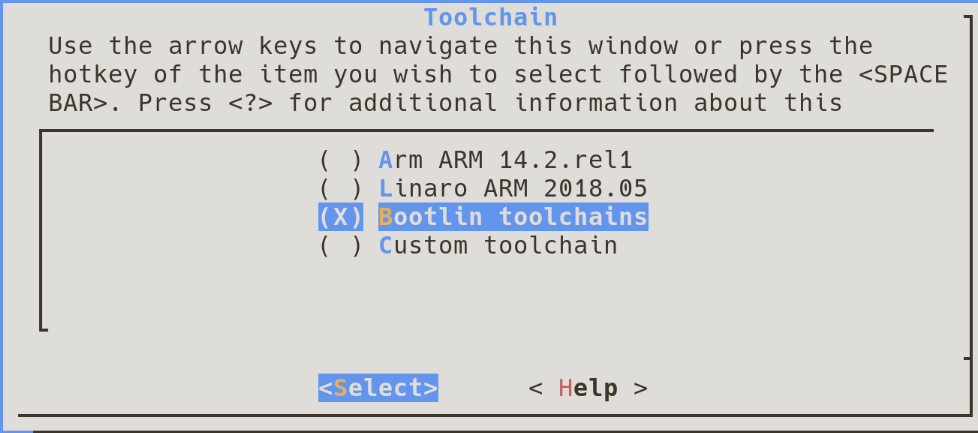
\includegraphics[width=\textwidth]{slides/buildroot-toolchain/external-toolchain-profiles.png}
  \end{columns}
\end{frame}

\begin{frame}{Existing external toolchains: Bootlin toolchains}
  \begin{columns}
    \column{0.6\textwidth}
    \begin{itemize}
    \item \url{https://toolchains.bootlin.com}
    \item A set of 218 pre-built toolchains, freely available
      \begin{itemize}
      \item 43 different CPU architecture variants
      \item All possible C libraries supported: glibc, uClibc-ng, musl
      \item Toolchains built with Buildroot!
      \end{itemize}
    \item Two versions for each toolchain
      \begin{itemize}
      \item {\em stable}, which uses the default version of gcc,
        binutils and gdb in Buildroot
      \item {\em bleeding-edge}, which uses the latest version of gcc,
        binutils and gdb in Buildroot
      \end{itemize}
    \item Directly integrated in Buildroot
    \end{itemize}
    \column{0.4\textwidth}
    \begin{center}
      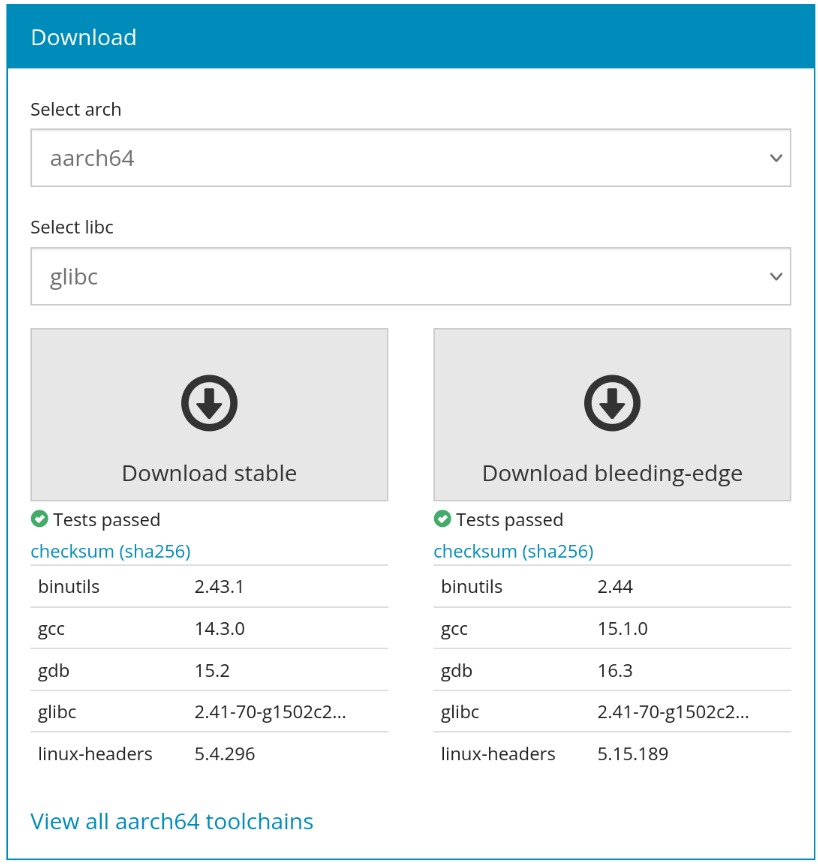
\includegraphics[height=0.5\textheight]{slides/buildroot-toolchain/bootlin-toolchains-com.png}
      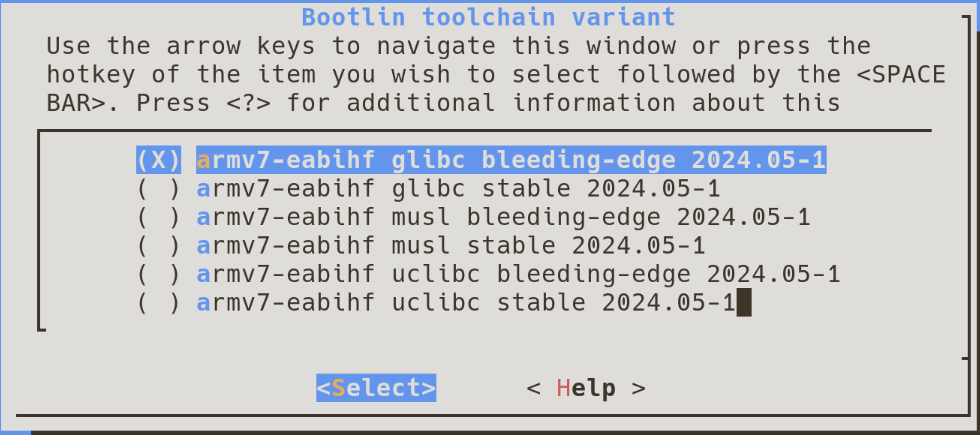
\includegraphics[width=0.8\textwidth]{slides/buildroot-toolchain/bootlin-toolchains-menuconfig.png}
    \end{center}
  \end{columns}

\end{frame}

\begin{frame}{Custom external toolchains}
  \begin{itemize}
  \item If you have a custom external toolchain, for example from your
    vendor, select \code{Custom toolchain} in \code{Toolchain}.
  \item Buildroot can download and extract it for you
    \begin{itemize}
    \item Convenient to share toolchains between several
      developers
    \item Option \code{Toolchain to be downloaded and
        installed} in \code{Toolchain origin}
    \item The URL of the toolchain tarball is needed
    \end{itemize}
  \item Or Buildroot can use an already installed toolchain
    \begin{itemize}
    \item Option \code{Pre-installed toolchain} in \code{Toolchain
        origin}
    \item The local path to the toolchain is needed
    \end{itemize}
  \item In both cases, you will have to tell Buildroot the
    configuration of the toolchain: C library, kernel headers version,
    etc.
    \begin{itemize}
    \item Buildroot needs this information to know which packages can
      be built with this toolchain
    \item Buildroot will check those values at the beginning of the
      build
    \end{itemize}
  \end{itemize}
\end{frame}

\begin{frame}{Custom external toolchain example configuration}
  \begin{center}
    \includegraphics[height=0.8\textheight]{slides/buildroot-toolchain/external-toolchain-config.png}
  \end{center}
\end{frame}

\begin{frame}{External toolchain: result}
  \begin{itemize}
  \item \code{host/opt/ext-toolchain}, where the original toolchain
    tarball is extracted. Except when a local pre-installed toolchain
    is used.
  \item \code{host/bin/<tuple>-<tool>}, symbolic links to the
    cross-compilation tools in their original location. Except the
    compiler, which points to a wrapper program.
  \item \code{host/<tuple>/}
    \begin{itemize}
    \item \code{sysroot/usr/include/}, the kernel headers and C
      library headers
    \item \code{sysroot/lib/} and \code{sysroot/usr/lib/}, C library and
      gcc runtime
    \item \code{include/c++/}, C++ library headers
    \end{itemize}
  \item \code{target/}
    \begin{itemize}
    \item \code{lib/} and \code{usr/lib/}, C and C++ libraries
    \end{itemize}
  \item The wrapper takes care of passing the appropriate flags to the
    compiler.
    \begin{itemize}
    \item Mimics the internal toolchain behavior
    \end{itemize}
  \end{itemize}
\end{frame}

\begin{frame}{Kernel headers version}
  \begin{itemize}
  \item One option in the toolchain menu is particularly important:
    the kernel headers version.
  \item When building user space programs, libraries or the C library,
    kernel headers are used to know how to interface with the kernel.
  \item This kernel/user space interface is {\bf backward compatible},
    but can introduce new features.
  \item It is therefore important to use kernel headers that have a
    version {\bf equal or older} than the kernel version running on
    the target.
  \item With the internal toolchain backend, choose an appropriate
    kernel headers version.
  \item With the external toolchain backend, beware when choosing your
    toolchain.
  \end{itemize}
\end{frame}

\begin{frame}{Other toolchain menu options}
  \begin{itemize}
  \item The toolchain menu offers a few other options:
    \begin{itemize}
    \item {\em Target optimizations}
      \begin{itemize}
      \item Allows to pass additional compiler flags when building
        target packages
      \item Do not pass flags to select a CPU or FPU, these are
        already passed by Buildroot
      \item Be careful with the flags you pass, they affect the entire
        build
      \end{itemize}
    \item {\em Target linker options}
      \begin{itemize}
      \item Allows to pass additional linker flags when building
        target packages
      \end{itemize}
    \item gdb/debugging related options
      \begin{itemize}
      \item Covered in our {\em Application development} section later.
      \end{itemize}
    \end{itemize}
  \end{itemize}
\end{frame}
